\documentclass[11pt]{article}

\usepackage[margin=1in]{geometry}
\usepackage[T1]{fontenc}
\usepackage{lmodern}
\usepackage{microtype}
\usepackage{booktabs}
\usepackage{tabularx}
\usepackage{enumitem}
\usepackage{amsmath}
\usepackage{graphicx}
\usepackage{float}
\usepackage{caption}
\usepackage[hidelinks]{hyperref}

\setlist{itemsep=2pt, topsep=4pt}
\setlength{\parskip}{4pt}
\captionsetup{font=small, labelfont=bf}
\graphicspath{{figs/}{../figs/}}

\title{\textbf{Rules vs.\ Learned Detectors: Auditing Data Quality in\\
San Diego's ``Get It Done'' 311 Service Requests}\\[4pt]
\large CS 677 Data Quality Assurance --- Final Project Report}
\author{Devashish Palate \and Mohammadreza Ghassemzadeh}
\date{December 2026}

\begin{document}
\maketitle

% =====================================================================
\begin{abstract}
\noindent
Municipal 311 records are used to judge how quickly a city responds to residents, so their defects become errors in public performance metrics. We audit the City of San Diego's ``Get It Done'' requests closed in 2025 (378,669 records, 23 columns). A suite of 14 executable quality rules finds few hard errors (255 records, 0.07\%), but a profiling step uncovers a date-granularity trap: because \texttt{date\_closed} has no time, a naive timestamp comparison flags 111,985 same-day closures (29.6\%) as ``closed before opened'', versus 4 genuine cases. We compare four families of detectors (declarative rules, a spatial nearest-neighbour consistency check, a duplicate detector, and two unsupervised outlier detectors, Isolation Forest and LOF) by injecting eight error types into a clean sample. Rules are perfect on the error types they encode and blind to everything else; Isolation Forest is the only detector that catches plausible-but-wrong response times (recall 0.98); LOF is weak across the board; and the spatial check and duplicate detector each cover a class that no other method sees. Against the City's own 41,999 duplicate labels, our duplicate detector reaches recall 0.72 at precision 0.32 on a held-out half-year, and inspection shows that the City links only a minority of obvious duplicates: we find 26,868 unlabeled high-confidence duplicates. Removing duplicates lowers mean days-to-close by 13\% (46.0 to 40.1) and reorders four of nine council districts; in contrast, the naive ``cleaning'' that falls into the timestamp trap triples the median (2 to 6 days) and reorders eight districts. The practical lesson is that a wrong cleaning rule can distort a metric more than the defects it targets.
\end{abstract}

% =====================================================================
\section{Problem Definition}

Residents of San Diego report potholes, graffiti, illegal dumping, and similar issues through the City's ``Get It Done'' app, website, and phone line. The City publishes every closed request on its open data portal~\cite{sdopendata}, and these records feed dashboards and comparisons of response time across the nine council districts. A duplicated report, an impossible date, or a record with the wrong district silently changes those comparisons.

We treat the dataset as a case study in comparing \emph{manual constraint-based} and \emph{automated} data quality assurance (course Weeks 3--8) and ask three questions:

\begin{description}[leftmargin=1.2cm, style=nextline]
  \item[RQ1] For each type of defect, how well do declarative quality rules, a spatial consistency check, a duplicate detector, and unsupervised outlier detectors (Isolation Forest, LOF) detect it?
  \item[RQ2] How accurately can a simple duplicate detector recover the duplicates the City has labeled, and what does it find that the City did not label?
  \item[RQ3] Does cleaning materially change response time per council district, including the ranking of districts?
\end{description}

% =====================================================================
\section{Dataset and Profiling}

\paragraph{Source.} ``Get It Done Requests closed in 2025'' from the City of San Diego Open Data Portal~\cite{sdopendata}: 378,669 records, one per service request, and 23 columns. Columns fall into identifiers (request ID, parent request ID, SAP notification number), time (\texttt{date\_requested} with a time of day, \texttt{date\_closed} as a date only, \texttt{case\_age\_days}), location (\texttt{lat}, \texttt{lng}, street address, zip code, council district, community plan), categories (service name and detail, status, case origin, record type), and free text (public description, referral note).

\paragraph{Profile.} We computed single-column statistics (completeness, distinct values, ranges, formats) and simple multi-column dependencies, following the profiling tasks surveyed by Abedjan et al.~\cite{abedjan2015profiling}. Table~\ref{tab:profile} summarizes the main findings. Status is either \emph{Closed} (350,711) or \emph{Referred} (27,958, handed to another agency, median age 0 days). 26,732 requests (7.1\%) were filed before 2025 and closed during it, some as early as 2016, so ``requests closed in 2025'' is a mix of new work and backlog. \texttt{case\_age\_days} always equals \texttt{date\_closed} minus the request \emph{day}, which confirms that the City computes age at day granularity. Three fields are mostly empty (park name 95.8\%, referral note 92.1\%, SAP number 87.6\%), and \texttt{service\_request\_parent\_id} is filled for exactly 41,999 records (11.1\%): these are the City's own duplicate labels, each pointing to the request it was merged into (the parent is present in the file for 94.8\% of them).

\begin{table}[tbp]
\centering\small
\caption{Key profiling results on the 2025 file.}
\label{tab:profile}
\begin{tabularx}{\linewidth}{@{}Xr@{}}
\toprule
Finding & Records \\
\midrule
City-labeled duplicates (non-null \texttt{service\_request\_parent\_id}) & 41,999 (11.1\%) \\
``Closed before opened'', naive timestamp comparison & 111,985 (29.6\%) \\
``Closed before opened'', compared at day granularity & 4 \\
Missing zip code / council district / coordinates & 7,024 / 1,233 / 399 \\
Coordinates outside the San Diego bounding box & 67 \\
Missing service name & 180 \\
Requested before 2025 (backlog closed in 2025) & 26,732 (7.1\%) \\
Median days to close: City duplicates vs.\ others & 12 vs.\ 2 \\
\bottomrule
\end{tabularx}
\end{table}

\paragraph{The date-granularity trap.} \texttt{date\_closed} is stored as \texttt{2025-04-01} while \texttt{date\_requested} is \texttt{2025-04-01 09:05:00}. Parsed naively, the close becomes midnight, earlier than the request, for every same-day closure. A validity rule written on full timestamps would therefore flag almost a third of the data. We compare all dates at day granularity and test that explicitly (Section~\ref{sec:rules}). Section~\ref{sec:rq3} shows what happens if an analyst ``cleans'' these rows away.

% =====================================================================
\section{Method}

The pipeline is written in Python (pandas, scikit-learn, pytest) and runs end to end in a few minutes on a laptop. Code is organized as one library (\texttt{dq.py}) and one script per stage.

\subsection{Quality rules as test assertions}
\label{sec:rules}

We encode 14 rules as executable checks organized by quality dimension, following the consumer-oriented dimensions of Wang and Strong~\cite{wang1996beyond} and the ``unit tests for data'' approach of Schelter et al.~\cite{schelter2018dq}. Each rule is a function that returns, per record, whether it is violated. The test suite has two parts: 28 \emph{unit tests} that check each rule fires on a hand-made bad record and stays silent on a good one (including a test that a same-day closure is \emph{not} a violation while the naive comparison flags it), and 14 \emph{data assertions} that run each rule against the real file. All unit tests pass; a failing data assertion is a documented defect (Table~\ref{tab:rules}).

\begin{table}[tbp]
\centering\small
\caption{Rule suite and violations on the full dataset (378,669 records).}
\label{tab:rules}
\begin{tabularx}{\linewidth}{@{}llXr@{}}
\toprule
Dimension & Rule & Definition & Violations \\
\midrule
Completeness & C1 & ID, request date, service, status, close date non-null & 180 \\
             & C2 & Latitude/longitude present & 399 \\
             & C3 & Council district present & 1,233 \\
             & C4 & Zip code present & 7,024 \\
Uniqueness   & U1 & \texttt{service\_request\_id} unique & 0 \\
Validity     & V1 & Coordinates inside San Diego bounding box & 67 \\
             & V2 & Council district in 1--9 & 0 \\
             & V3 & Zip code in 91900--92199 & 5 \\
             & V4 & Status in \{Closed, Referred\} & 0 \\
Consistency  & K1 & day(\texttt{date\_requested}) $\le$ \texttt{date\_closed} & 4 \\
             & K2 & \texttt{case\_age\_days} = \texttt{date\_closed} $-$ day(\texttt{date\_requested}) & 0 \\
Timeliness   & T1 & \texttt{date\_closed} within 2025 & 0 \\
             & T2 & Requested on/after Get It Done launch (May 2016) & 0 \\
             & T3 & \texttt{case\_age\_days} $\ge 0$ & 4 \\
\bottomrule
\end{tabularx}
\end{table}

The 67 out-of-bounds points include four at (0,\,0) (``null island''), two with a flipped longitude sign (+117), and several in other states (e.g.\ Pittsburgh, Chicago), consistent with device geolocation errors. The five invalid zips include 94103 and 94124 (San Francisco) and 12341.

\subsection{Spatial consistency check}

Without network access to district boundary files, we replace the planned point-in-polygon test with a nearest-neighbour vote: a record is flagged if at least 80\% of its 15 nearest neighbours (haversine distance) carry a different council district. On the full file this flags 337 records.

\subsection{Unsupervised outlier detection}

Isolation Forest~\cite{liu2008iforest} (200 trees) and Local Outlier Factor~\cite{breunig2000lof} ($k=20$) run on nine standardized features: latitude, longitude, signed $\log(1+\text{age})$, age relative to the median for the same service type, request hour, day of week, fractional request year, and frequency encodings of service type and district. Missing values are median-imputed. Each detector flags the top 5\% of anomaly scores; we also report threshold-free average precision.

\subsection{Duplicate detection}

Following standard record-linkage practice~\cite{elmagarmid2007duplicate}, we generate candidate pairs by blocking on a $\sim$50\,m grid cell (plus neighbouring cells), keep pairs within 50\,m and 180 days, and apply a \emph{temporal overlap} constraint: the later request must be filed on or before the earlier one was closed. Profiling showed that 99.8\% of City-labeled pairs satisfy this, because a report can only be merged into an open request; the constraint removes 72\% of candidates while keeping 99.9\% of true pairs. Each pair gets a score from spatial closeness (weight 0.30), temporal closeness $e^{-\Delta t/14\text{d}}$ (0.20), same service type (0.30), and token-set similarity of address and description (0.10 each). The later record of any pair above a threshold is predicted to be a duplicate.

\subsection{Cleaning}

Cleaning proceeds in logged, cumulative stages: S1 removes records violating hard rules (C1, V1, V3, K1, T3: 255 records); S2 removes City-labeled duplicates (41,993); S3 removes high-confidence unlabeled duplicates filed by residents (16,185; see Section~\ref{sec:rq2}); S4 imputes missing districts (750) and reassigns spatially inconsistent ones (313) by nearest-neighbour vote. For comparison, a \emph{naive} cleaning drops every ``closed before opened'' record using full timestamps (111,985 records).

% =====================================================================
\section{Experimental Results}

\subsection{RQ1: Which detector catches which defect?}
\label{sec:rq1}

Real errors have no complete ground truth, so we draw a clean pool of 328,915 records (passing all rules, not a City duplicate, not spatially flagged), sample 40,000 per run, and inject one error type at a time at 1\% and 5\% of records, over five random seeds (80 runs). Encodings and the spatial reference are fit on the remaining clean records, disjoint from the sample. The eight error types are: missing required field (service name or status set to null); impossible date (closed 1--30 days before request); out-of-bounds coordinates (null island, flipped sign, or elsewhere in the US); swapped latitude/longitude; invalid district (0, 10, 11, 99); wrong-but-valid district (another value in 1--9); inflated response (request date pushed 1--4 years earlier with a consistent case age, so every rule still passes); and near-duplicate (a copy filed 5\,min--72\,h later, $\sim$9\,m away, while the original is open).

\begin{figure}[tbp]
\centering
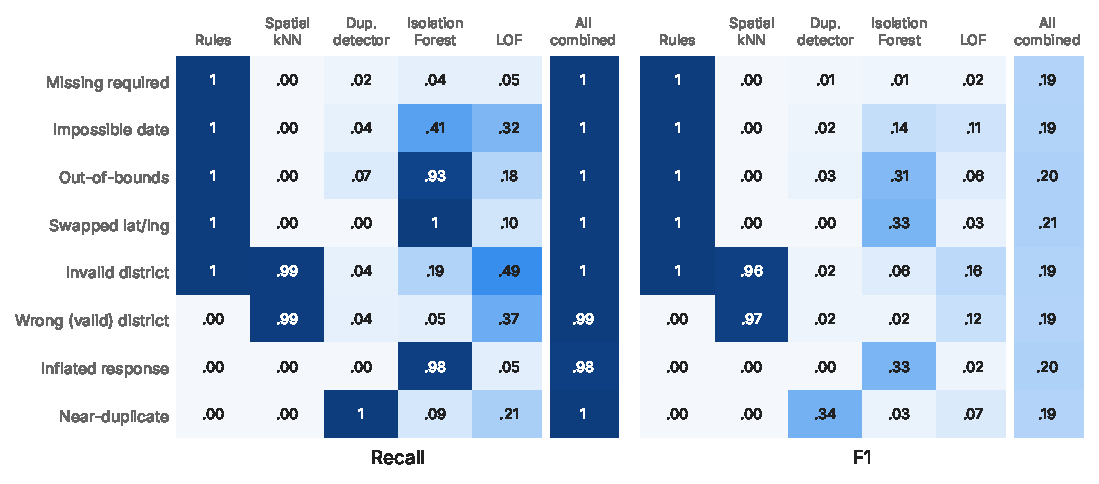
\includegraphics[width=\linewidth]{injection_heatmap}
\caption{Recall and F1 per injected error type (rows) and detector (columns) (1\% of records injected; IF and LOF flag the top 5\%; mean of five seeds). Rules are perfect on what they encode and blind elsewhere; each other detector owns one class.}
\label{fig:heat}
\end{figure}

\newcommand{\INFLIF}{0.98}
\newcommand{\WRONGKNN}{0.99}
\newcommand{\DUPREC}{1.00}
\begin{table}[tbp]
\centering\scriptsize
\caption{Precision / recall / F1 per detector and error type, 1\% of records injected (mean of five seeds, all s.d.\ $\le$ 0.04). IF and LOF flag a fixed 5\% of records, so their precision is capped at 0.20. Bold: best F1 per error type. 5\% results are in \texttt{injection\_summary.csv}.}
\label{tab:inj}
\setlength{\tabcolsep}{4pt}
\begin{tabular}{@{}lccccc@{}}
\toprule
Error type & Rules & kNN & Dup. & IF & LOF \\
\midrule
Missing required & \textbf{1.00/1.00/1.00} & 0.00/0.00/0.00 & 0.01/0.02/0.01 & 0.01/0.04/0.01 & 0.01/0.05/0.02 \\
Impossible date & \textbf{1.00/1.00/1.00} & 0.02/0.00/0.00 & 0.01/0.04/0.02 & 0.08/0.41/0.14 & 0.06/0.32/0.11 \\
Out-of-bounds & \textbf{1.00/1.00/1.00} & 0.00/0.00/0.00 & 0.02/0.07/0.03 & 0.19/0.93/0.31 & 0.04/0.18/0.06 \\
Swapped lat/lng & \textbf{1.00/1.00/1.00} & 0.00/0.00/0.00 & 0.00/0.00/0.00 & 0.20/1.00/0.33 & 0.02/0.10/0.03 \\
Invalid district & \textbf{1.00/1.00/1.00} & 0.94/0.99/0.96 & 0.01/0.04/0.02 & 0.04/0.19/0.06 & 0.10/0.49/0.16 \\
Wrong (valid) district & 0.00/0.00/0.00 & \textbf{0.94/0.99/0.97} & 0.01/0.04/0.02 & 0.01/0.05/0.02 & 0.07/0.37/0.12 \\
Inflated response & 0.00/0.00/0.00 & 0.02/0.00/0.00 & 0.00/0.00/0.00 & \textbf{0.20/0.98/0.33} & 0.01/0.05/0.02 \\
Near-duplicate & 0.00/0.00/0.00 & 0.03/0.00/0.00 & \textbf{0.21/1.00/0.34} & 0.02/0.09/0.03 & 0.04/0.21/0.07 \\
\bottomrule
\end{tabular}
\end{table}


We treat 1\% as the main setting because real error rates in this file are below 1\%, and give the ML detectors a review budget of 5\% of records. At a 5\% injection rate the budget equals the number of errors, so ML precision and recall coincide by construction (both shown in \texttt{injection\_summary.csv}). Figure~\ref{fig:heat} and Table~\ref{tab:inj} show a clean division of labour:
\begin{itemize}
  \item \textbf{Rules} reach recall 1.00 with no false alarms on the five error types they encode (missing, impossible date, out-of-bounds, swapped, invalid district) and recall 0 on the three they do not. Their precision is 1.00 by construction here, because the clean pool already passes every rule.
  \item \textbf{Isolation Forest} is the only detector that catches \emph{inflated response} errors (\INFLIF{} recall), the case that passes every rule because it is internally consistent. It also catches all swapped and 93\% of out-of-bounds coordinates, but always with lower precision than rules, because its review budget is filled with genuine but unusual records (old backlog cases, rare service types). Its average precision on inflated responses is only 0.39 at the 1\% rate (0.70 at 5\%; Figure~\ref{fig:ap}): the injected records land inside the top 5\% of scores but mixed with genuine unusual records, so a tighter review budget would catch fewer. When errors make up 5\% of records, the same budget catches 0.71 of them.
  \item \textbf{LOF} is weak on every type (best recall 0.49, on invalid districts). Local density is a poor fit here: injected values are often global outliers in a single feature, which Isolation Forest isolates quickly, while LOF's neighbourhoods are dominated by the dense urban core.
  \item The \textbf{spatial check} is the only method that finds a \emph{wrong but valid} district (\WRONGKNN{} recall at precision 0.94); no rule can, because the value is in the valid domain.
  \item The \textbf{duplicate detector} is the only method that finds near-duplicates (\DUPREC{} recall); rules see a new unique ID and outlier detectors see a perfectly normal record. Its precision is low (0.21) because the ``clean'' pool still contains unlabeled real duplicates, the same effect we measure in RQ2.
\end{itemize}
Combining rules, the spatial check, the duplicate detector, and Isolation Forest reaches recall $\ge$0.98 on all eight types (Figure~\ref{fig:heat}, last column); without Isolation Forest, inflated responses are missed entirely. The combination's precision (about 0.10 at 1\%) is limited by Isolation Forest's review budget, whose flags an analyst would review rather than delete.

\begin{figure}[tbp]
\centering
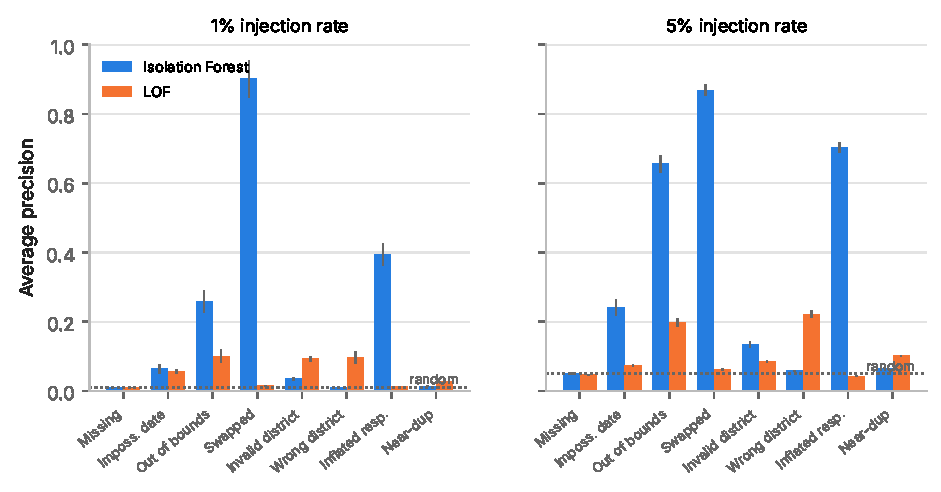
\includegraphics[width=\linewidth]{ml_avg_precision}
\caption{Threshold-free average precision of the two ML detectors per error type (mean $\pm$ s.d.\ over five seeds); the dotted line is a random ranking.}
\label{fig:ap}
\end{figure}

\subsection{RQ2: Recovering the City's duplicate labels}
\label{sec:rq2}

We tune the threshold on requests closed January--June 2025 (best F1 at 0.70) and evaluate on July--December. On the held-out half, the detector flags 48,195 records with \textbf{recall 0.72, precision 0.32, F1 0.45} (training half: 0.70 / 0.30 / 0.42). Blocking keeps 83\% of labeled pairs; the rest are more than 50\,m apart (12\%), more than 180 days apart, or different service types (8\%). Precision stays near 0.33 at every threshold (Figure~\ref{fig:dup}), which suggests the ``false positives'' are not random noise.

\begin{figure}[tbp]
\centering
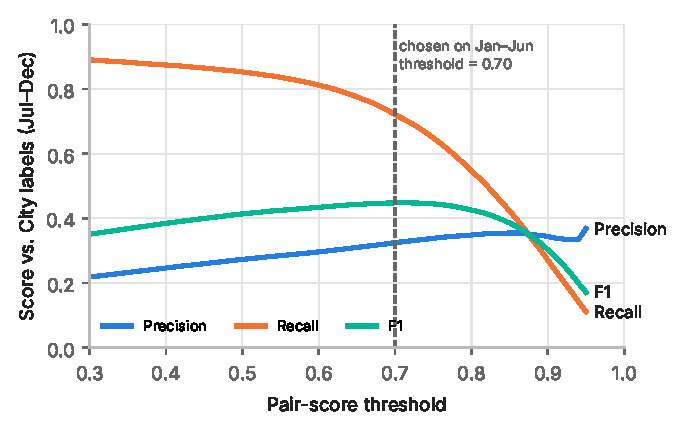
\includegraphics[width=0.62\linewidth]{dup_sweep}
\caption{Duplicate detection vs.\ City labels on the July--December hold-out, by threshold.}
\label{fig:dup}
\end{figure}

To test this, we apply a strict definition of an obvious duplicate: same service type, at most 15\,m apart, filed within 24 hours while the earlier request was open. 38,246 records meet it, and only 11,378 of them carry a City label, leaving \textbf{26,868 unlabeled high-confidence duplicates}. Conversely, only 27\% of City-labeled duplicates meet the strict definition, so the City also merges reports that are farther apart in space or time. Inspection of a random sample of unlabeled pairs shows two groups: clear resident duplicates (same address, minutes apart, closed together), and crew-generated tickets (``Crew/Self Generated'' and ``Worker App'' origins, about 39\% of the unlabeled group) that log each graffiti tag or illegal-dumping pile as a separate work item. We therefore count the City's labels as an \emph{incomplete} reference: measured precision is a lower bound, and for cleaning we remove only the 16,185 strict duplicates filed through resident channels (app, web, phone, email).

\subsection{RQ3: Does cleaning change the district comparison?}
\label{sec:rq3}

Table~\ref{tab:clean} and Figure~\ref{fig:district} report days-to-close by council district before and after cleaning (all statuses; results for Closed-only are similar).

\begin{table}[tbp]
\centering\small
\caption{Days to close by council district. Medians use whole days; bootstrap 95\% CIs for the raw medians are at most $\pm$1 day.}
\label{tab:clean}
\begin{tabular}{@{}lrrrrrr@{}}
\toprule
 & \multicolumn{3}{c}{Median} & \multicolumn{3}{c}{Mean} \\
\cmidrule(lr){2-4}\cmidrule(l){5-7}
District & Raw & Cleaned & Naive & Raw & Cleaned & Naive \\
\midrule
1 & 2 & 2 & 6 & 59.8 & 51.7 & 83.6 \\
2 & 2 & 2 & 6 & 52.9 & 46.1 & 74.6 \\
3 & 2 & 2 & 5 & 48.6 & 40.5 & 69.5 \\
4 & 2 & 2 & 7 & 36.1 & 32.1 & 53.1 \\
5 & 5 & 4 & 7 & 60.2 & 52.3 & 72.7 \\
6 & 5 & 4 & 8 & 40.2 & 38.4 & 49.3 \\
7 & 3 & 3 & 7 & 44.0 & 41.9 & 57.9 \\
8 & 2 & 2 & 7 & 34.2 & 30.2 & 51.8 \\
9 & 2 & 1 & 6 & 43.0 & 37.4 & 64.4 \\
\midrule
City & 2 & 2 & 6 & 46.0 & 40.1 & 65.3 \\
\bottomrule
\end{tabular}
\end{table}

\begin{figure}[tbp]
\centering
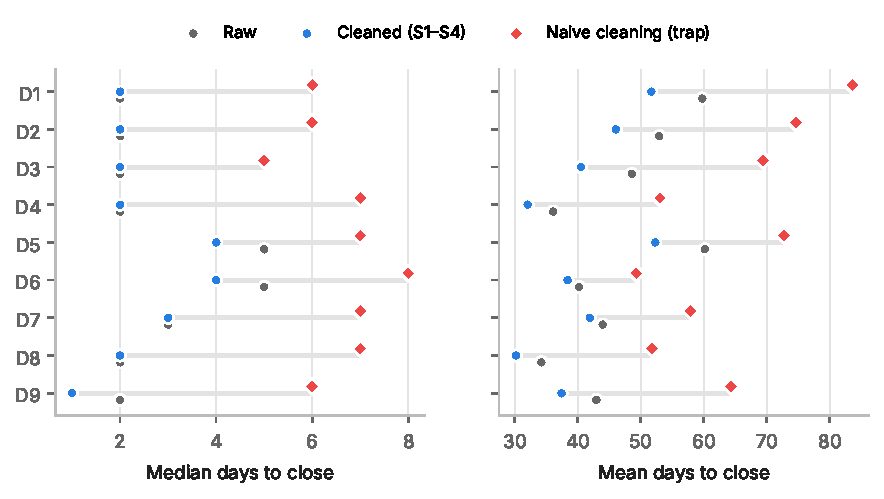
\includegraphics[width=\linewidth]{district_response}
\caption{Median and mean days to close per council district: raw, after cleaning stages S1--S4, and after the naive timestamp-based cleaning.}
\label{fig:district}
\end{figure}

\begin{itemize}
  \item \textbf{Rule violations barely matter.} Removing the 255 hard-error records changes no district value and no ranking.
  \item \textbf{Duplicates matter.} City-labeled duplicates have a median age of 12 days versus 2 for other records, because a merged report is closed only when its parent is. Removing them lowers the citywide mean from 46.0 to 39.2 days, and full cleaning ends at 40.1 (S3 removes short-lived resident duplicates, which raises the mean slightly). Medians move by one day in Districts 5, 6, and 9. Ranking districts by mean, four of nine change position (Kendall $\tau = 0.89$).
  \item \textbf{The wrong cleaning rule matters most.} Dropping ``closed before opened'' records by full timestamp removes 29.6\% of the data, almost all of it same-day closures. The citywide median triples (2 to 6 days), the mean rises by 42\%, and eight of nine districts change rank (median $\tau = 0.65$). For example, Districts 5 and 6 tie as slowest by raw median (5 days), but after the naive cleaning District 6 is clearly slowest (8) and District 5 ties with Districts 4, 7, and 8 (7).
\end{itemize}

\begin{figure}[tbp]
\centering
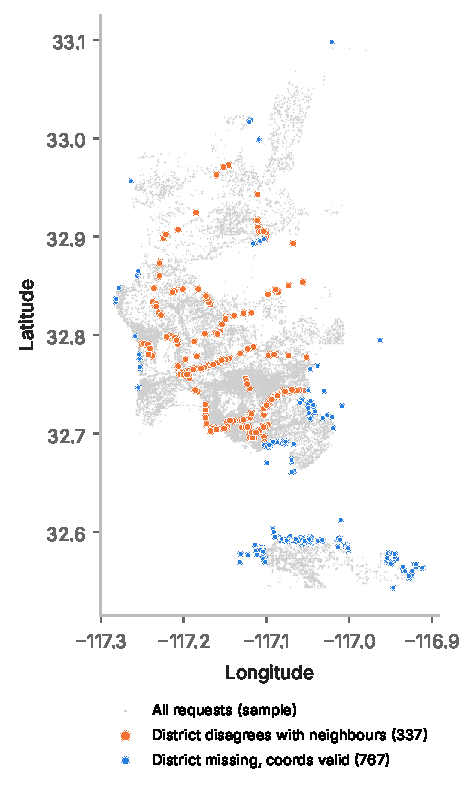
\includegraphics[width=0.4\linewidth]{map_flags}
\caption{Records whose district disagrees with $\ge$80\% of their 15 nearest neighbours (orange) cluster along district boundaries; records with valid coordinates but no district (blue) sit at the city's edges.}
\label{fig:map}
\end{figure}

% =====================================================================
\section{Discussion}

\paragraph{Rules vs.\ learned detectors.} The two families are complements, not competitors. Rules are exact, explainable, and free of false alarms, but only for defects someone anticipated. Unsupervised detectors find defects nobody wrote a rule for, here the internally consistent but implausible response time, at the cost of a fixed review budget full of genuine-but-unusual records. Two defect classes (wrong-but-valid district, near-duplicates) need neither: they need \emph{relational} checks that compare a record with its neighbours in space or time. For practitioners, the most useful order is rules first, relational checks second, and an Isolation Forest review queue last.

\paragraph{Profiling before rules.} The most consequential finding came from profiling, not from any detector: the date-granularity mismatch. A rule written without checking the field's format would have generated 111,985 false violations, and acting on them would have distorted every downstream metric more than all real defects combined.

\paragraph{Limitations.}
\begin{itemize}
  \item \emph{Injected errors} follow our assumptions about how errors look; real errors may be subtler or correlated. Rule precision of 1.00 is partly by construction, since the clean pool passes every rule.
  \item \emph{The City's duplicate labels are incomplete}, so precision in RQ2 is a lower bound, and our ``high-confidence'' duplicates are a heuristic, not verified ground truth; crew-generated tickets in particular may be legitimate separate work items.
  \item \emph{The spatial check is a proxy} for a point-in-polygon test. Its flags concentrate on district boundaries (Figure~\ref{fig:map}), where nearest neighbours legitimately disagree, and missing-district records at the city edge may lie outside city limits, so imputing a district for them may be wrong.
  \item \emph{Response time is measured in whole days}, so medians are coarse and many districts tie; mean-based rankings are more sensitive.
  \item \emph{ML thresholds}: the fixed 5\% budget is arbitrary; average precision (Figure~\ref{fig:ap}) gives a threshold-free view.
\end{itemize}

\paragraph{Future work.} Replace the kNN proxy with official council district polygons; adjudicate a labeled sample of duplicate pairs to estimate true precision; extend to the time-series view (course Weeks 9--10) by detecting anomalous daily request volumes per service type; and analyse Referred cases separately, since their near-zero ages measure hand-off speed rather than resolution.

% =====================================================================
\section{Conclusion}

On 378,669 San Diego 311 requests, explicit quality rules found few hard errors, profiling exposed a format trap affecting 30\% of rows, and an injection study showed that rules, relational checks, and unsupervised detectors each catch distinct defect classes. Duplicates, which the City labels only partially, shift district response-time comparisons by about 13\%, while a single mis-specified cleaning rule triples the median. Data quality work on public metrics should therefore start with profiling, encode what is known as tests, and use learned detectors to find what nobody anticipated.

% =====================================================================
\begin{thebibliography}{9}

\bibitem{wang1996beyond}
R.~Y. Wang and D.~M. Strong.
Beyond accuracy: What data quality means to data consumers.
\emph{Journal of Management Information Systems}, 12(4):5--33, 1996.

\bibitem{abedjan2015profiling}
Z.~Abedjan, L.~Golab, and F.~Naumann.
Profiling relational data: A survey.
\emph{The VLDB Journal}, 24(4):557--581, 2015.

\bibitem{schelter2018dq}
S.~Schelter, D.~Lange, P.~Schmidt, M.~Celikel, F.~Biessmann, and A.~Grafberger.
Automating large-scale data quality verification.
\emph{Proceedings of the VLDB Endowment}, 11(12):1781--1794, 2018.

\bibitem{liu2008iforest}
F.~T. Liu, K.~M. Ting, and Z.-H. Zhou.
Isolation forest.
In \emph{Proc.\ IEEE International Conference on Data Mining (ICDM)}, pages 413--422, 2008.

\bibitem{breunig2000lof}
M.~M. Breunig, H.-P. Kriegel, R.~T. Ng, and J.~Sander.
LOF: Identifying density-based local outliers.
In \emph{Proc.\ ACM SIGMOD International Conference on Management of Data}, pages 93--104, 2000.

\bibitem{elmagarmid2007duplicate}
A.~K. Elmagarmid, P.~G. Ipeirotis, and V.~S. Verykios.
Duplicate record detection: A survey.
\emph{IEEE Transactions on Knowledge and Data Engineering}, 19(1):1--16, 2007.

\bibitem{sdopendata}
City of San Diego.
Get It Done requests closed in 2025.
City of San Diego Open Data Portal.
\url{https://data.sandiego.gov}. Accessed November 2026.

\end{thebibliography}

\end{document}
